\documentclass[11pt]{amsart}          
\usepackage[a4paper,verbose]{geometry}
\geometry{top=3cm,bottom=3cm,left=3cm,right=3cm,textheight=595pt}
\setlength{\parskip}{0.3em}
% ==============================
% PACKAGES
% ==============================

\usepackage{amsfonts}
\usepackage{amssymb}  
\usepackage{amsthm} 
\usepackage{amsmath} 
\usepackage{caption}
\usepackage[inline]{enumitem}
\setlist{itemsep=0em, topsep=0em, parsep=0em}
\setlist[enumerate]{label=(\alph*)}
\usepackage{etoolbox}
\usepackage{stmaryrd} 
\usepackage[dvipsnames]{xcolor}
\usepackage[]{hyperref}
\hypersetup{
  colorlinks,
  linkcolor=blue,
  citecolor=blue,
  urlcolor=blue}
\usepackage{graphicx}
\graphicspath{{assets/}}
\usepackage{mathtools}

\usepackage{tikz-cd}
\usepackage{minted}
\usepackage{float}
\usetikzlibrary{
  matrix,
  arrows,
  shapes
}

\newcommand{\rr}{{\mathbb{R}}}
\newcommand{\nn}{{\mathbb{N}}}
\newcommand{\iso}{\cong}
\newcommand{\too}{\longrightarrow}
\newcommand{\tto}{\rightrightarrows}
\newcommand{\To}[1]{\xrightarrow{#1}}
\newcommand{\Too}[1]{\To{\;\;#1\;\;}}
\newcommand{\from}{\leftarrow}
\newcommand{\From}[1]{\xleftarrow{#1}}
\newcommand{\Cat}[1]{\mathbf{#1}}
\newcommand{\cat}[1]{\mathcal{#1}}
\newtheorem*{remark}{Remark}
\renewcommand{\ss}{\subseteq}
\newcommand{\hask}[1]{\mintinline{Haskell}{#1}}
\newenvironment{haskell}
  {\VerbatimEnvironment
  	\begin{minted}[escapeinside=??, mathescape=true,frame=single, framesep=5pt, tabsize=1]{Haskell}}
  {\end{minted}}

\author{Bartosz Milewski}
\title{Initial algebra as a directed colimit}

\begin{document}
\maketitle{}

There is a a piece of folklore about algebras in Haskell, which says that both the initial algebra and the terminal coalgebra for a given functor are defined by the same fixed point formula. This works for most common cases, but is not true in general. What is definitely true is that they are both fixed points--this result is called the Lambek's lemma--but there may be many fixed points. The initial algebra is the \textit{least fixed point}, and the terminal coalgebra is the \textit{greatest fixed point}.

In this series of blog posts I will explore the ways one can construct these (co-)algebras using category theory and illustrate it with Haskell examples. 

In this first installment, I'll go over the construction of the initial algebra.
\section{A functor}
Let's start with a simple functor that generates binary trees. Normally, we would store some additional data in a tree (meaning, the functor would take another argument), either in nodes or in leaves, but here we're just interested in pure shapes.

\begin{haskell}
data F a = Leaf 
         | Node a a
  deriving Show
\end{haskell}
Categorically, this functor can be written as a \textit{coproduct} of the terminal object $1$ and the \textit{product} of $a$ with itself, here written simply as $a^2$
\[F a = 1 + a^2\]
The lifting of functions is given by this implementation of \hask{fmap}
\begin{haskell}
instance Functor F where
  fmap _ Leaf       = Leaf
  fmap f (Node x y) = Node (f x) (f y)
\end{haskell}

We can use this functor to build arbitrary level trees. Let's consider, for instance, terms of type \hask{F Int}. We can either build a \hask{Leaf} or a \hask{Node} with two numbers in it
\begin{haskell}
x1, y1 :: F Int
x1 = Leaf
y1 = Node 1 2
\end{haskell}
With those, we can build next-level values of the type $F^2 a$ or, in our case, \hask{F (F Int)}
\begin{haskell}
x2, y2 :: F (F Int)
x2 = Leaf
y2 = Node x1 y1
\end{haskell}
We can display \hask{y2} directly using \hask{show}
\begin{haskell}
> Node Leaf (Node 1 2)
\end{haskell}
or draw the corresponding tree
\begin{figure}[H]
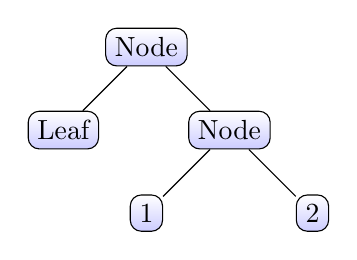
\begin{tikzpicture}[
    level distance=3em,
  every node/.style = {shape=rectangle, rounded corners,
    draw, align=center,
    top color=white, bottom color=blue!20}]
    \tikzstyle{level 1}=[sibling distance=6em]
    \tikzstyle{level 2}=[sibling distance=6em]
  \node {Node}
    child { node {Leaf}  }
    child { node {Node}
      child { node {$1$} }
      child { node {$2$} } };
\end{tikzpicture}
\end{figure}
Since $F$ is an endofunctor, so is $F^2$. Lifting a function $f \colon a \to b$ to $F^2$ can be implemented by applying \hask{fmap} twice. Here's the action of \hask{(+1)} on our test values
\begin{haskell}
fmap (fmap (+1)) x2
> Leaf
fmap (fmap (+1)) y2
> Node Leaf (Node 2 3)
\end{haskell}
or, graphically,
\begin{figure}[H]
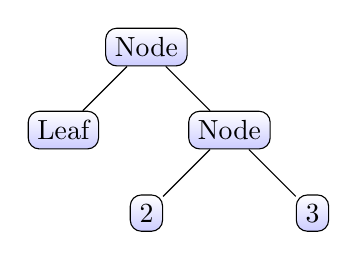
\begin{tikzpicture}[
    level distance=3em,
  every node/.style = {shape=rectangle, rounded corners,
    draw, align=center,
    top color=white, bottom color=blue!20}]
    \tikzstyle{level 1}=[sibling distance=6em]
    \tikzstyle{level 2}=[sibling distance=6em]
  \node {Node}
    child { node {Leaf}  }
    child { node {Node}
      child { node {$2$} }
      child { node {$3$} } };
\end{tikzpicture}
\end{figure}

You can see that \hask{Leaf}s at any level remain untouched; only the contents of bottom \hask{Node}s in the tree are transformed.

\section{The colimit construction}

The carrier of the initial algebra can be constructed as a colimit of an infinite sequence. This sequence is constructed by applying powers of $F$ to the initial object which we'll denote as $0$. We'll see how this works first in our example.

The initial object in Haskell is defined as a type with no data constructor (we are ignoring the question of non-termination in Haskell). 
\begin{haskell}
data Void
  deriving Show
\end{haskell}
In Set, this is just an empty set.

The \hask{Show} instance for \hask{Void} requires the pragma
\begin{haskell}
{-# language EmptyDataDeriving #-}
\end{haskell}
Even though there are no values of the type \hask{Void}, we can still construct a value of the type \hask{F Void}
\begin{haskell}
z1 :: F Void
z1 = Leaf
\end{haskell}
This degenerate version of a tree can be drawn as
\begin{figure}[H]
\centering
\centering
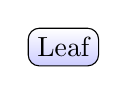
\begin{tikzpicture}[
  every node/.style = {shape=rectangle, rounded corners,
    draw, align=center,
    top color=white, bottom color=blue!20}]
  \node {Leaf};
\end{tikzpicture}
\end{figure}

This illustrates a very important property of our $F$: Its action on an empty set does not produce an empty set. This is what allows us to generate a non-trivial sequence of powers of $F$ starting with the empty set. 

Not every functor has this property. For instance, the construction of the initial algebra for the functor
\begin{haskell}
data StreamF a x = ConsF a x
\end{haskell}
will produce an uninhabited type (empty set). This is different from its terminal coalgebra, which is an infinite stream
\begin{haskell}
data Stream a = Cons a (Stream a)
\end{haskell}

Double application of our \hask{F} to \hask{Void} produces, again, a \hask{Leaf}, as well as a \hask{Node} that contains two \hask{Leaf}s. 
\begin{haskell}
z2, v2 :: F (F Void)
z2 = Leaf

v2 = Node z1 z1
> Node Leaf Leaf
\end{haskell}
Graphically,
\begin{figure}[H]
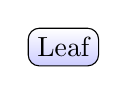
\begin{tikzpicture}[
  every node/.style = {shape=rectangle, rounded corners,
    draw, align=center,
    top color=white, bottom color=blue!20}]
  \node {Leaf};
\end{tikzpicture}
\qquad
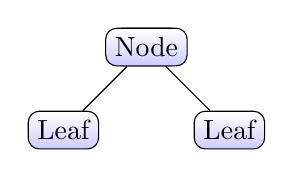
\begin{tikzpicture}[
    level distance=3em,
  every node/.style = {shape=rectangle, rounded corners,
    draw, align=center,
    top color=white, bottom color=blue!20}]
    \tikzstyle{level 1}=[sibling distance=6em]
  \node{Leaf};
  \node {Node}
    child { node {Leaf} }
    child { node {Leaf} };
\end{tikzpicture}
\end{figure}
In general, powers of $F$ acting on \hask{Void} generate trees which terminate with \hask{Leaf}s (but there can be no terminal \hask{Node}s). Higher and higher powers of $F$ acting on \hask{Void} will eventually produce any tree we can think of. But for any given power, there will exist even larger trees that are not generated by it. 

In order to get all the trees we could take a sum (a coproduct) of infinitely many powers. Something like this
\[\sum_{n = 0}^{\infty} F^n 0\]
The problem is that we'd also get a lot of duplication. For instance, we saw that \hask{z1} was the same tree as \hask{z2}. In general, a \hask{Leaf} is produced at all non-zero powers of $F$ acting on \hask{Void}. Similarly, all powers of $F$ greater than one produce a single node with two leaves, and so on.

We have to have a way of identifying multiply generated trees. This is why we need a \textit{colimit} rather than a simple coproduct. 

As a reminder, a coproduct is defined as a universal cocone. Here, the base of the cocone is the set of all powers of $F$ acting on $0$ (Haskell \hask{Void}).

\begin{figure}[H]
\centering
\begin{tikzcd}
  0
   \arrow[dr, "\iota_0"']
   &F 0
   \arrow[d, "\iota_{(F 0)}"]
   &F^2 0
   \arrow[dl, "\iota_{(F^2 0)}"]
   & ...
   \\
   &\sum_{n = 0}^{\infty} F^n 0
\end{tikzcd}
\end{figure}
In a more general colimit, the objects in the base of the cocone may be connected by morphisms. 

Coming from the initial object, there can be only one morphism. We'll call this morphism $!$ or, in Haskell, \hask{absurd}
\begin{haskell}
absurd :: Void -> a
absurd a = case a of {}
\end{haskell}
This definition requires another pragma
\begin{haskell}
{-# language EmptyCase #-}
\end{haskell}
We can construct a morphism from $F 0$ to $F^2 0$ as a lifting $F !$. In Haskell, the lifting of \hask{absurd} doesn't change the shape of trees. Here it is acting on a leaf
\begin{haskell}
z1' :: F (F Void)
z1' = fmap absurd z1
> Leaf
\end{haskell}
We can continue this process of lifting \hask{absurd} to higher and higher powers of $F$
\begin{haskell}
z2', v2' :: F (F (F Void))

z2' = fmap (fmap absurd) z2
> Leaf

v2' = fmap (fmap absurd) v2
> Node Leaf Leaf
\end{haskell}
We can construct an infinite chain (this kind of directed chain index by natural numbers is called an $\omega$-chain)
\begin{figure}[H]
\centering
\begin{tikzcd}
  0
  \arrow[r, "!"]
   &F 0
   \arrow[r, "F !"]
   &F^2 0
   \arrow[r, dashed]
   & ...
\end{tikzcd}
\end{figure}
We can use this chain as the base of a cocone. The colimit of this chain is defined as the universal cocone. We will call the apex of this cocone $\mu F$
\begin{figure}[H]
\centering
\begin{tikzcd}
  0
  \arrow[r, "!"]
   \arrow[d, "\iota_0"]
   &F 0
   \arrow[r, "F !"]
   \arrow[dl, "\iota_{(F 0)}"]
   &F^2 0
   \arrow[r, dashed]
   \arrow[dll, bend left, "\iota_{(F^2 0)}"]
   & ...
   \\
   \mu F
\end{tikzcd}
\end{figure}
In $Set$ these constructions have simple interpretations. A coproduct is a discriminated union. A colimit is a discriminated union in which we identify all the injections that are connected by morphisms in the base of the cocone. For instance
\[\iota_0 = \iota_{(F 0)}\, \circ \, !\]
\[\iota_{(F 0)} =   \iota_{(F^2 0)} \circ  F !\]
and so on.

Here we use the lifted \hask{absurd} (or $!$ in the picture above) as the morphisms that connect the powers of $F$ acting of \hask{Void} (or $0$ in the picture). 

These are exactly the identifications that we were looking for. For instance, $F !$ maps the leaf generated by $F 0$ to the leaf which is the element of $F^2 0$. Or, translating it to Haskell, \hask{(fmap absurd)} maps the leaf generated by \hask{F Void} to the leaf generated by \hask{F (F Void)}, and so on. 

All trees generated by the $n$'th power of $F$ are injected into the $n+1$'st power of $F$ by \hask{absurd} lifted by the $n$th power of $F$. 

The colimit is formed by equivalence classes with respect to these identifications. In particular, there is a class for a degenerate tree consisting of a single leaf whose representative can be taken from \hask{F Void}, or from \hask{F (F Void)}, or from \hask{F (F (F Void))} and so on. 

\section{Initiality}

The colimit $\mu F$ is exactly the initial algebra for the functor $F$. This follows from the universal property of the colimit. First we will show that for any algebra $(A, \alpha \colon F A \to A)$ there is a unique morphism from $\mu F$ to $A$. Indeed, we can build a cocone with $A$ at its apex and the injections given by 
\[!\]
\[\alpha \circ F !\]
\[\alpha \circ F \alpha \circ F^2 !\]
and so on

\begin{figure}[H]
\centering
\begin{tikzcd}
  0
  \arrow[r, "!"]
  \arrow[d, "!"]
   &F 0
   \arrow[r, "F !"]
  \arrow[d, "F !"]
   &F^2 0
   \arrow[r, dashed]
  \arrow[d, "F^2 !"]
   & ...
   \\
  A
   &F A
   \arrow[l, "\alpha"]
   &F^2 A
   \arrow[l, "F \alpha"]
   & ...
   \arrow[l, dashed]
\end{tikzcd}
\end{figure}

Since the colimit $\mu F$ is defined by the universal cocone, there is a unique morphism from it to $A$. It can be shown that this morphism is in fact an algebra morphism. This morphism is called a \textit{catamorphism}.

\section{Fixed Point}

Lambek's lemma states that the initial algebra is a fixed point of the functor that defines it
\[F (\mu F) \cong \mu F\]
This can also be seen directly, by applying the functor to every object and morphism in the $\omega$-chain that defines the colimit. We get a new chain that starts at $F 0$
\begin{figure}[H]
\centering
\begin{tikzcd}
   F 0
   \arrow[r, "F !"]
   &F^2 0
   \arrow[r, "F^2 !"]
   &F^3 0
   \arrow[r, dashed]
   & ...
\end{tikzcd}
\end{figure}
But the colimit of this chain is the same as the colimit $\mu F$ of the original chain. This is becuase we can always add back the initial object to the chain, and define its injection $\iota_0$ as the composite  
\[\iota_0 = F ! \circ \iota_{(F 0)} \]
On the other hand, if we apply $F$ to the whole universal cocone, we'll get a new cocone with the apex $F (\mu F)$. In principle, this cocone doesn't have to be universal, so we cannot be sure that $F (\mu F)$ is a colimit. If it is, we say that $F$ \textit{preserves} the particular type of colimit---here, an $\omega$-colimit. 

Remember: the image of a cocone under a functor is always a cocone (this follows from functoriality). Preservation of colimits is an additional requirement that the image of a \textit{universal} cocone be \textit{universal}. 

The result is that, if $F$ preserves $\omega$-colimits, then the initial algebra $\mu F$ is a fixed point of $F$
\[F(\mu F) \cong \mu F\]
because both sides can be obtained as a colimit of the same $\omega$-chain. 

\section{Bibliography}
\begin{itemize}
\item Ad\'amek, Milius, Moss, \href{https://www8.cs.fau.de/staff/milius/publications/files/CoalgebraBook.pdf}{Initial Algebras, Terminal Coalgebras, and
the Theory of Fixed Points of Functors}
\end{itemize}

\end{document}
\maketitle{}